\documentclass[CJK]{beamer}
\usepackage{CJKutf8}
\usepackage{xcolor} % 使用颜色宏包
\usepackage{listings}
\lstset{
lang ge=C,
numbers=left,
numbersep=5pt,
TAB frame=single,
breaklines=true,                % 自动断行
breakatwhitespace=false,        % 断行只在空格处
}
\usetheme{Copenhagen}
\setbeamercovered{transparent}
\begin{document}
\begin{CJK*}{UTF8}{gbsn}

\title{Reflections on Trusting Trust}
\subtitle{\tiny To what extent should one trust a statement that a program is free of Trojan horses?\\ Perhaps it is more important to trust the people who wrote the software.}
\author{夏永锋}
\institute[SJTU]{上海交通大学\ 软件学院\\嵌入式实验室}
\date{\today}

\begin{frame}
	\titlepage
\end{frame}

\begin{frame}{About Ken}
\begin{columns}
	\column{2cm}
	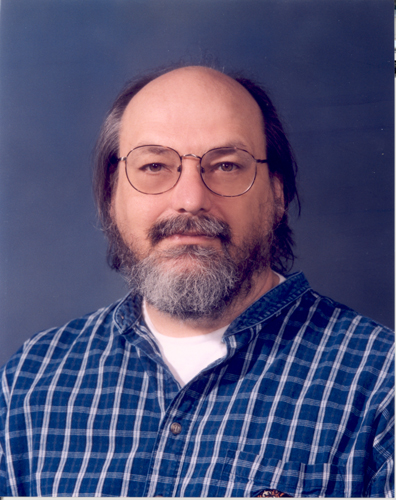
\includegraphics[width=2cm]{Ken.jpg}
	\column{9cm}
		\begin{itemize}
			
			\item Born in New Orleans in 1943
			\item Received a Bachelor of Science in 1965 and a master's degree in 1966, both in Electrical Engineering and Computer Science, from the University of California, Berkeley
			\item Retired from Bell Labs in late 2000, then worked at Entrisphere,Inc as a fellow until 2006
			\item Now works at Google as a Distinguished Engineer.
			
		\end{itemize}
\end{columns}
\end{frame}
{\tiny
\begin{frame}{About Ken}
	\begin{block}{Contributions}
		\begin{itemize}
			\item the Bon programming language
			\item one of the creators and early developers of the the Unix and Plan 9 operating system
			\item the B programming language, a precursor to Ritchie's C
			\item participate in  creating C programming language
			\item Regular expressions and early computer text editors QED and ed
			\item most recently the co-creation of Google's programming language Go
			\item developed UTF-8 together with Rob Pike in 1992
			\item participate in creating endgame tablebases and the chess machine Belle
		\end{itemize}
	\end{block}
	\begin{block}{Awards}	
		\begin{itemize}
			\item 1983, Turing Award
			\item 1990, IEEE Richard W. Hamming Medal
			\item 1997, Fellow of the Computer History Museum
			\item 1999, National Medal of Technology
			\item 1999, The first IEEE Tsutomu Kanai Award
			\item 2011, The Japan Prize for Information and Communication
		\end{itemize}
	\end{block}
\end{frame}
}
\begin{frame}{About Ken's Turing Award acceptance speech}
	\begin{quote}
	"Reflections on Trusting Trust" presented the backdoor attack now known as the {\color{red} Thompson hack} or {\color{red} trusting trust attack}, and is widely considered a seminal computer security work in its own right.
	\end{quote}
	\begin{flushright}
	--- From en.wikipedia.org
	\end{flushright}
\end{frame}
\begin{frame}{Why not to talk about UNIX?}
	\begin{itemize}
		\item UNIX swept into popularity with an industry-wide change from central mainframes to autonomous minis.
		\item The current state of UNIX is the result of the labors of a large number of people.
		\item I have not worked on mainstream UNIX in many years.
	\end{itemize}
	\begin{block}{}
	\begin{center}
	So what to talk about?\\
	The cutest program I ever wrote. and do this in three stages and bring it together at the end.
	\end{center}
	\end{block}
\end{frame}

{\tiny
\begin{lstlisting}[language=C,caption=Stage I "a self-reproducing program",label=ccode,keywordstyle=\color{blue!70}, commentstyle=\color{red!50!green!50!blue!50}, frame=shadowbox, rulesepcolor=\color{red!20!green!20!blue!20}]
char s[]={
	'\t',
	'0',
	'\n',
	'}',
	';',
	'\n',
	'\n',
	'/',
	'*',
	'\n',
	(213 line deleted)
	0
};

/*
 * The string s is a
 * representation of the body
 * of this program from '0'
 * to the end.
 */

main()
{
	int i;
	
	printf("char s[]={\n");
	for(i=0; s[i]; i++)
		printf("\t%d,\n",s[i]);
	printf("%s",s);
}
\end{lstlisting}
}

\begin{frame}{About the self-reproducing program}
	\begin{itemize}
		\item This program can be easily written by another program.
		\item This program can contain an arbitrary amount of excess baggage that will be reproduced along with th main algorithm.
	\end{itemize}
\end{frame}

{\tiny
\begin{lstlisting}[language=C,caption=Stage II 2.1,keywordstyle=\color{blue!70}, commentstyle=\color{red!50!green!50!blue!50}, frame=shadowbox, rulesepcolor=\color{red!20!green!20!blue!20}]
...
c=next();
if(c!='\\')
	return(c);
c=next();
if(c=='\\')
	return('\\');
if(c=='n')
	return('\n');
...
\end{lstlisting}
\begin{lstlisting}[language=C,caption=Stage II 2.2,keywordstyle=\color{blue!70}, commentstyle=\color{red!50!green!50!blue!50}, frame=shadowbox, rulesepcolor=\color{red!20!green!20!blue!20}]
...
c=next();
if(c!='\\')
	return(c);
c=next();
if(c=='\\')
	return('\\');
if(c=='n')
	return('\n');
if(c=='v')
	return('\v');
...
\end{lstlisting}
}

\begin{frame}{About Stage II}
Since the binary version of the compiler does not know about "$\setminus$v",the source is not legal C. We must "train" the compiler.\\
After it "knows" what "$\setminus$v" means, then our new change will become legal C.
\begin{block}{}
We look up on an ASCII chart that a vertical tab is decimal 11.
\end{block}
\end{frame}
{\tiny
\begin{lstlisting}[language=C,caption=Stage II 2.3,keywordstyle=\color{blue!70}, commentstyle=\color{red!50!green!50!blue!50}, frame=shadowbox, rulesepcolor=\color{red!20!green!20!blue!20}]
...
c=next();
if(c!='\\')
	return(c);
c=next();
if(c=='\\')
	return('\\');
if(c=='n')
	return('\n');
if(c=='v')
	return(11);
...
\end{lstlisting}
}
Now the old compiler accepts the new source.We install the resulting binary as the new official C compiler and now we can write the portable version the way we had it in Listing 3.
{\tiny
\begin{lstlisting}[language=C,caption=Stage III 3.1,keywordstyle=\color{blue!70}, commentstyle=\color{red!50!green!50!blue!50}, frame=shadowbox, rulesepcolor=\color{red!20!green!20!blue!20}]
compile(s)
char *s;
{
	...
}
\end{lstlisting}
}
\begin{frame}{About Stage III}
	\begin{block}{}
	Listing 5 represents the high level control of the C compiler where the routine "compile" is called to compile the next line of source.
	\end{block}
	\begin{block}{}
	Listing 6 shows a simple modification to the compiler that will deliberately miscompile source whenever a particular pattern is matched. If this were not deliberate,it would be called a compiler "bug". Since it is deliberate, it should be called a "Trojian horse".
	\end{block}
\end{frame}
{\tiny
\begin{lstlisting}[language=C,caption=Stage III 3.2,keywordstyle=\color{blue!70}, commentstyle=\color{red!50!green!50!blue!50}, frame=shadowbox, rulesepcolor=\color{red!20!green!20!blue!20}]
compile(s)
char *s;
{
	if(match(s,"pattern")){
		compile("bug");
		return;
	}
	...
}
\end{lstlisting}
The actual bug I planted in the compiler would match code in the UNIX "login" command. The replacement code would miscompile the login command so that it would accept either the intended encrypted password or a particular known password.\\
Such blatant code would not go undetected for long.Even the most casual perusal of the source of the C compiler would raise suspicions.
\begin{lstlisting}[language=C,caption=Stage III 3.3,keywordstyle=\color{blue!70}, commentstyle=\color{red!50!green!50!blue!50}, frame=shadowbox, rulesepcolor=\color{red!20!green!20!blue!20}]
compile(s)
char *s;
{
	if(match(s,"pattern1")){
		compile("bug1");
		return;
	}
	if(match(s,"pattern2")){
		compile("bug2");
		return;
	}
	...
}
\end{lstlisting}
}

\begin{frame}{Explain Listing 7}
In Listing 7, I simply adds a second Trojan horse to the one that already exists.
\begin{block}{}
{\bf The second pattern is aimed at the C compiler.}The replacement code is a Stage I self-reproducing program that inserts both Trojian horses into the compiler.
\end{block}
\begin{block}{}
This requires a learning phase as in the Stage II example.
	\begin{enumerate}
		\item We compile the modified source with the normal C compiler to produce a bugged binary.
		\item We install this binary as the official C.
		\item We can now remove the bugs from the source of the compiler and the new binary will reinsert the bugs whenever it is compiled.
	\end{enumerate}
\end{block}
Of course, the login command will remain bugged with no trace in source anywhere.
\end{frame}
\begin{frame}
	\begin{center}
	{\LARGE THANK YOU !}
	\end{center}
%	\begin{block}{}
%	\begin{center}
%	{\small Proud to use \LaTeX\ and Beamer.}
%	\end{center}
%	\end{block}
\end{frame}
\end{CJK*}
\end{document}